\newgeometry{left=17mm, right=17mm, top=8mm, bottom=13mm}
\chapter{ДВОРОВЫЕ КОМПАНИИ\protect\footnote{Многие данные и фотографии предоставлены мне Т. В. Меньшиковой. Ей же благодарен за добрые советы.}}

\noindent
Мне поручили написать о дворовых компанях, что я и постараюсь сделать с учетом <<собирательных>> свойств нашего Дома за период с тридцатых до шестидесятых годов. Аналог этого книжного варианта, естественно, будет в Альбоме.

Нельзя не сказать, что среди первопоселенцев нашего дома было очень много замечательных людей, начиная с Народного Комиссара иностранных дел М. М. Литвинова, его заместителей, руководителей подразделений, Послов того времени: Дивильковский И. А., Карский М.А., Майский И.М., Рубинин Е.В., Уманский К.А.

Сейчас, через 80 с лишним лет после заселения нашего дома, трудно сказать насколько были дружны между собой первопоселенцы, были ли дворовые компании у их старших детей (до 1920 года рождения)\footnote{Среди них, например: Клейн Н., Кунин В., Моргунова Т., Рабинович Э., Рубинин П.}, привлекались ли в эти компании ребята из других домов, что было характерно для последующих поколений, когда компании формировались из ребят окрестных дворов, как правило, в возрастном диапазоне 2-3 года с вкраплениями до 5 лет.

Собирательная особенность нашего двора наметилась еще до Войны, у ребят около 1924 года рождения, в основном выпускников школ 1941 года. К ним относятся участники ВОВ: Багун Ю., Варзар Сева, Дивильковский Юра, Клейн Наташа, Короткин Жора, Кунина Ляля, Миникс Аба.

\restoregeometry

\newgeometry{left=10mm, right=10mm, top=8mm, bottom=5mm}

\begin{figure}[h]
    \begin{minipage}{90mm}
        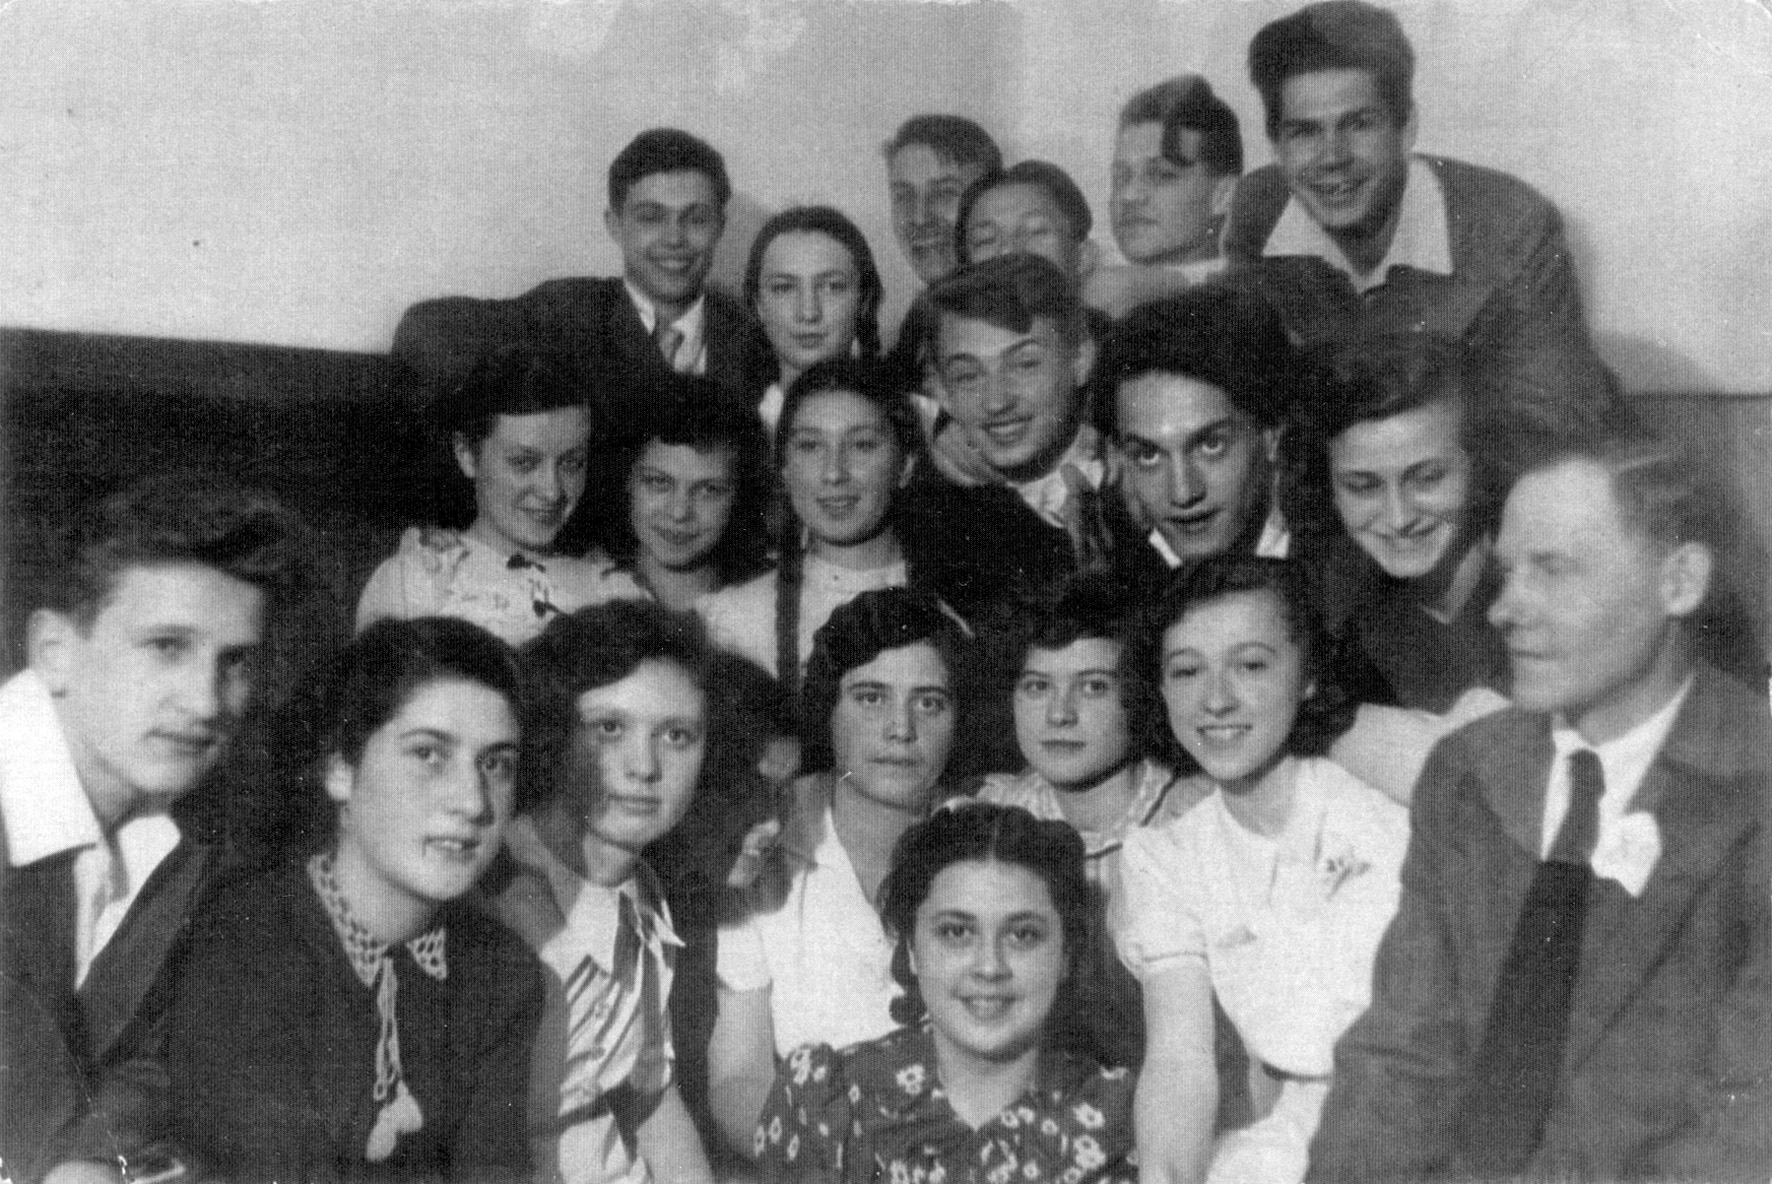
\includegraphics[width=90mm]{inc/MalDev}
        \textit{\footnotesize{Выпускники 10Б класса. 1941 год.}}
    \end{minipage}
\end{figure}

\vfill

\begin{figure}[h!]
    \begin{minipage}{73mm}
    \begin{minipage}[h!]{34mm}
        \center{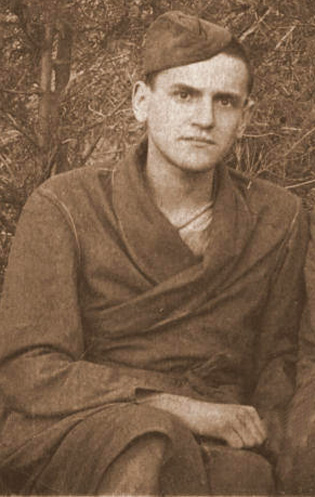
\includegraphics[width=\linewidth]{inc/24} }
    \end{minipage}
    \hspace{3mm}
    \begin{minipage}[h!]{34mm}
        \center{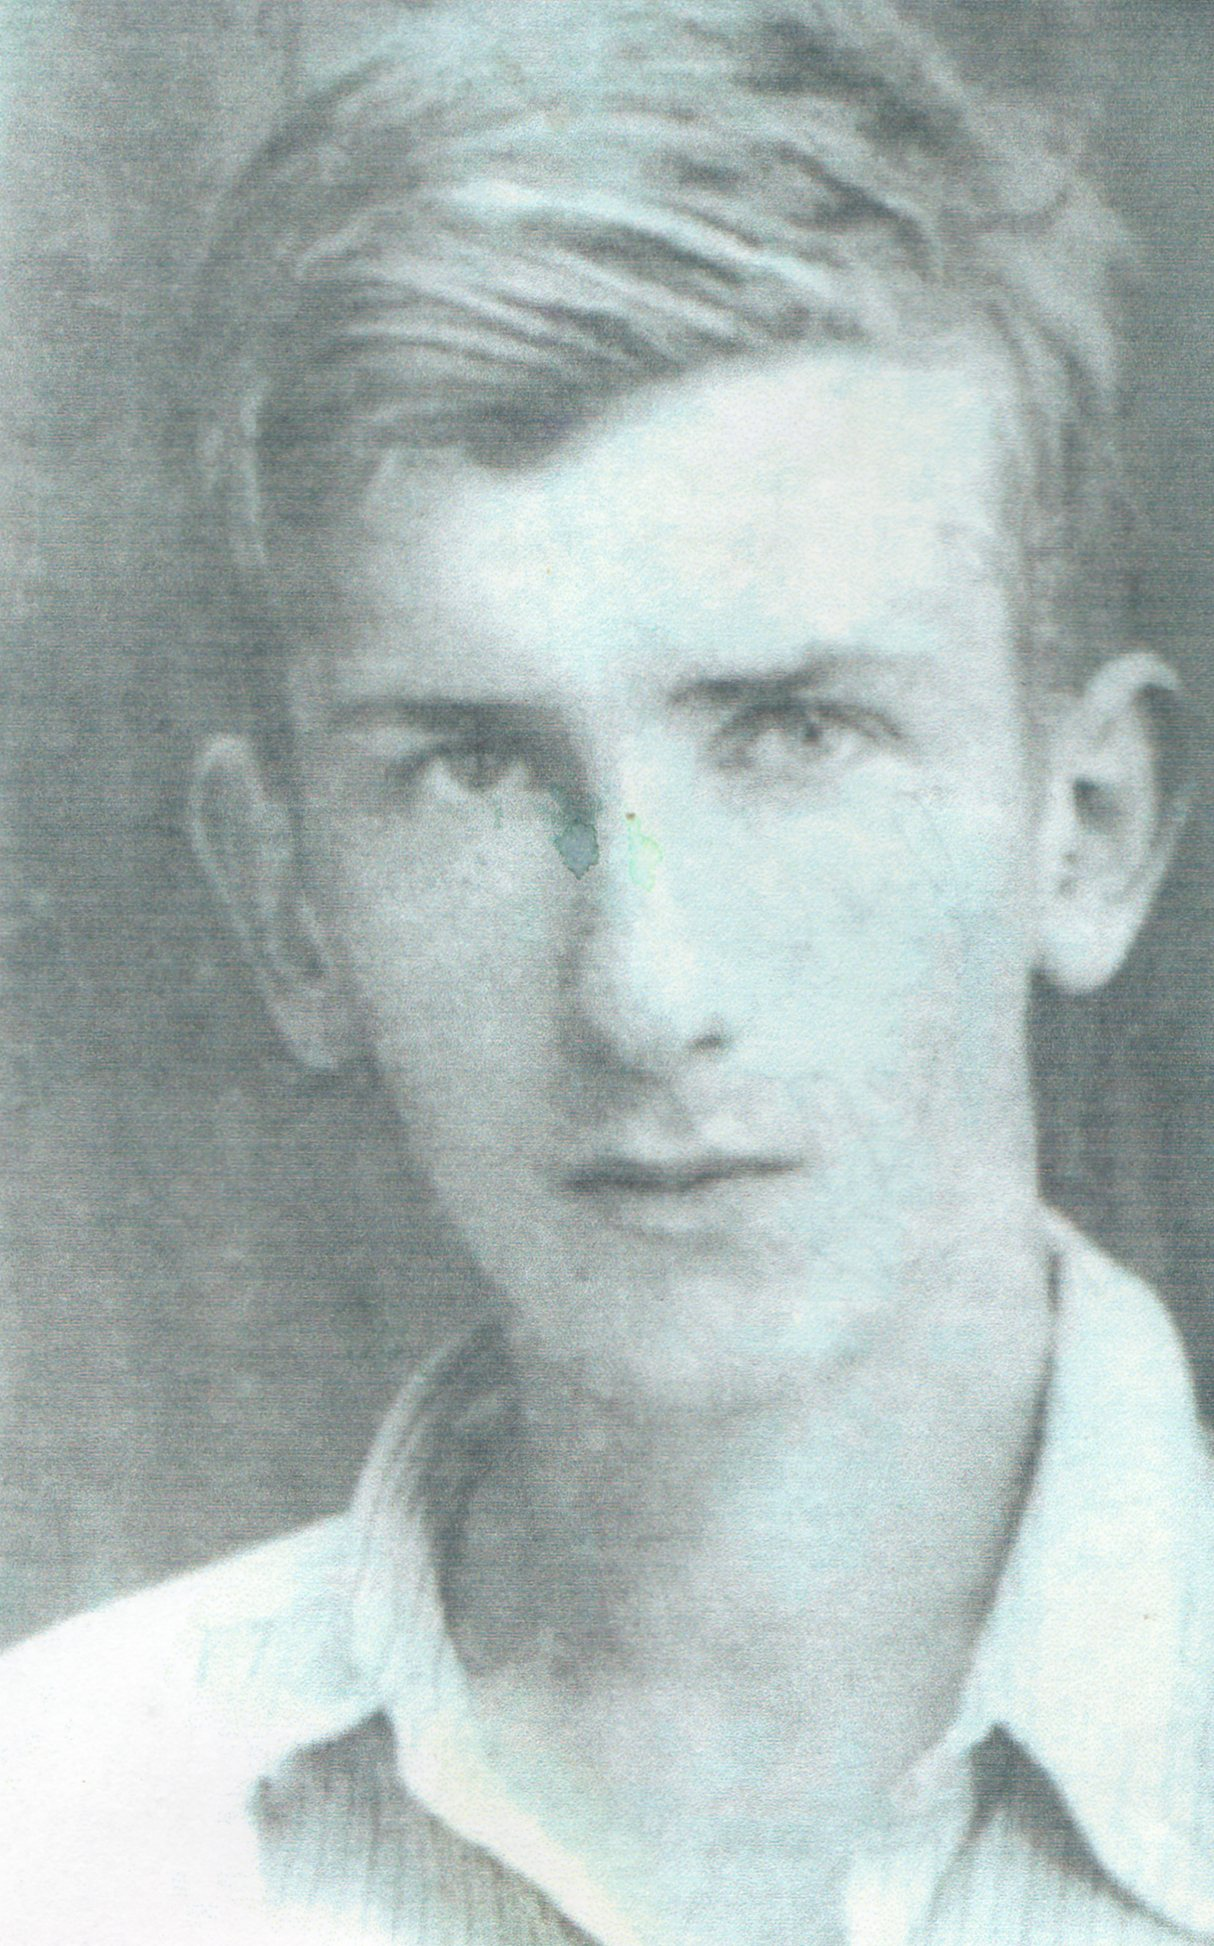
\includegraphics[width=\linewidth]{inc/RG027} }
    \end{minipage}    
    \vspace{-20pt}
    
    \textit{\footnotesize{Аба Миникс и Юра Дивильковский погибли на войне}}
    \end{minipage}
\end{figure}

\vfill

\begin{figure}[h!]
    \begin{minipage}{75mm}
        \begin{minipage}[h!]{34mm}
            \center{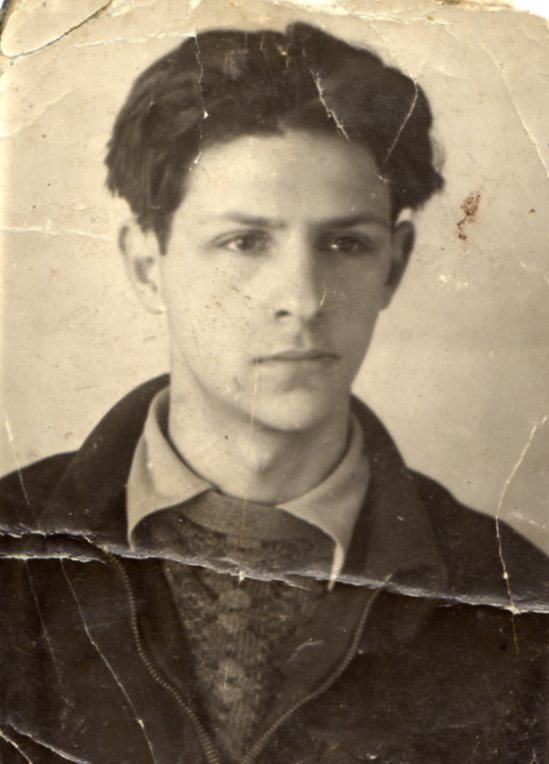
\includegraphics[width=\linewidth]{inc/RG024} }
        \end{minipage}
        \hspace{3mm}
        \begin{minipage}[h!]{36mm}
            \center{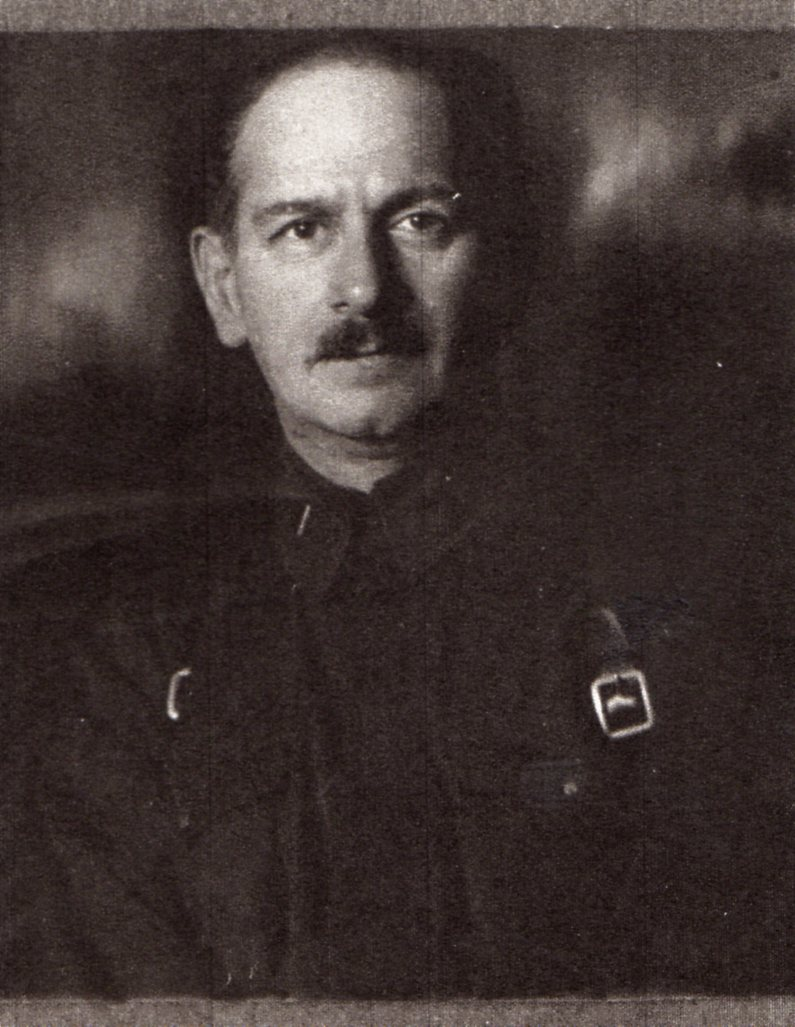
\includegraphics[width=\linewidth]{inc/RG026} }
        \end{minipage}
      
      
        \vspace{-10pt}
        \textit{\footnotesize{Отец и сын Короткины. Воевали на разных фронтах. Переписывались. Жора погиб. Отец выжил.}}  
     %\hspace{5pt}
      
    \end{minipage}
    \hspace{3mm}
    \begin{minipage}[h!]{37mm}
        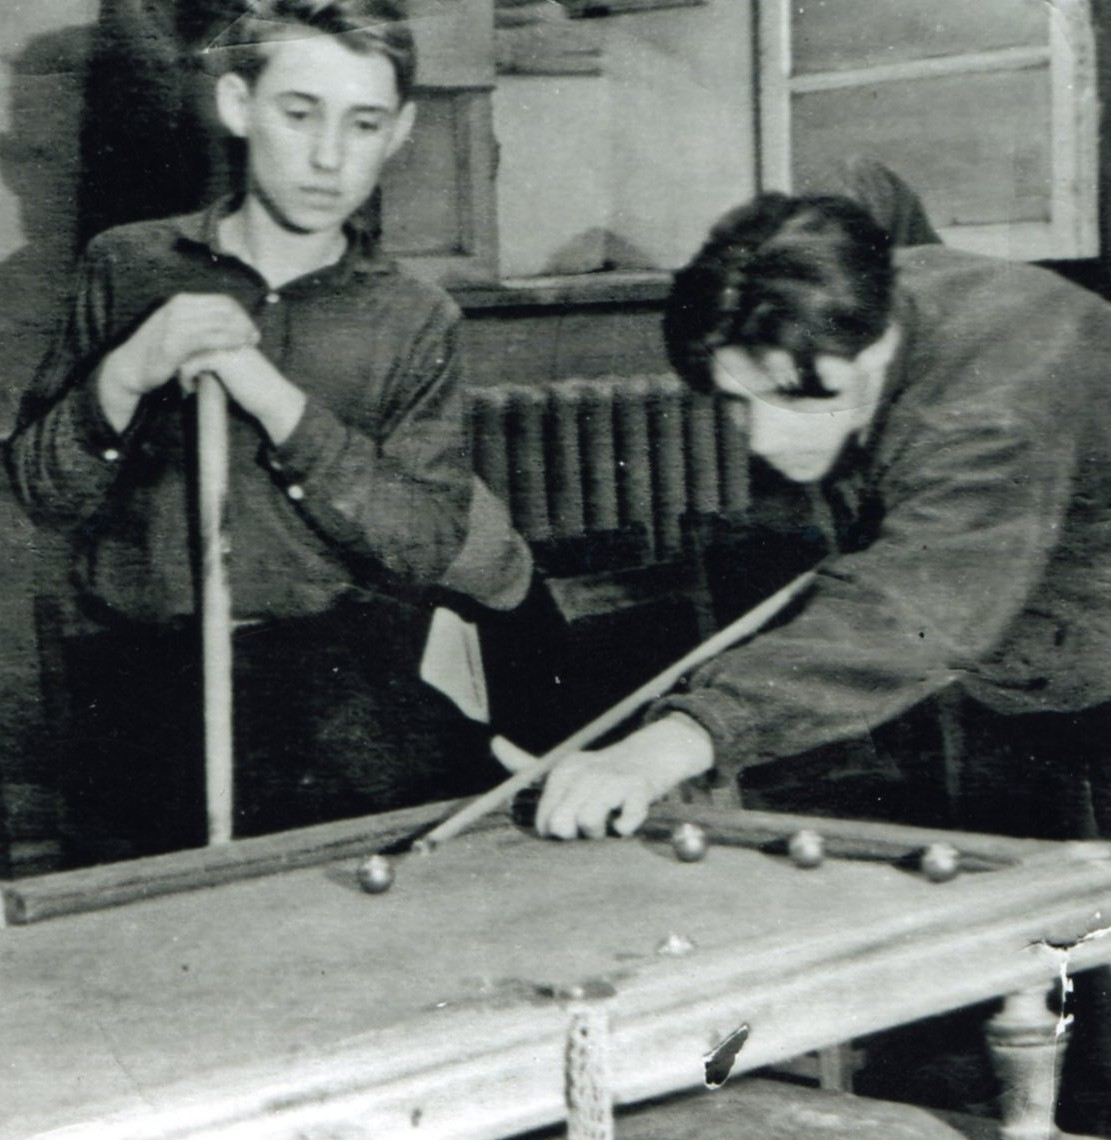
\includegraphics[width=\linewidth]{inc/RG025a}
        
        \vspace{-10pt}
        \textit{\footnotesize{Сева Варзар прошел всю войну, Жора Короткин~-- погиб.}}
    \end{minipage}
      
      
\end{figure}

\newpage % ??
\newgeometry{left=10mm, right=10mm, top=5mm, bottom=0mm}


\begin{small}

\begin{multicols}{2}
    
\itshape
    
    \noindent
    К ребятам нашего двора \\
    Пришла не лучшая пора. \\
    \vfill
    \noindent
    Груз годов ведь с плеч не скинешь,\\
    И, куда не поглядишь,\\
    Всюду виден, вроде, фииниш,\\
    И осталось, вроде, шиш! \\
    \vfill
    \noindent
    Только нам, знать, срок не вышел,\\
    Только порох, видно, есть,\\
    Коли вновь мы, братцы, здесь,\\
    Коль мы снова тут, под крышей\\
    Дома номер два дробь шесть.\\
    \vfill
    \noindent
    Откуда шли, шпана дворовая,\\
    Когда пришла пора суровая\\
    Расстаться, шумною толпой\\
    В жизнь, как на праздник~-- \\
    \indent 
    пей да пой!,--\\
    Ушли веселую шурьбой.\\
    Да каждый со своей судьбой.\\
    \vfill
    \noindent
    Пошли, в цепочку растянувшись,\\
    Один, едва начав, споткнувшись,\\
    Далече не успел уйти\\
    По незавдному пути;\\
    Другой, гляди, взлетел высоко,\\
    А третий ускакал далеко...\\
    \vfill   
    \noindent 
    А мир для всех куда как шире;\\
    В иных домах на нашей жизни \\ \indent ткань:\\
    То~-- шелк с парчей, то~-- просто \\ \indent дрянь!\\
    То планов дрезких грамадье,\\
    То только старое тряпье.\\
    \vfill
    \noindent
    Но жизнь~-- от Бога и надолго.\\
    И не забыть бы, братцы, долга\\
    За нами~-- тем, кто нас родил,\\
    Да тем, кто раньше уходил.\\
    Но не в прекрасную страну,\\
    А на проклятую войну.\\
    \vfill
    \noindent
    Утащила злая баба,\\
    Уложила в поле сдуру\\
    Твоео братишку Абу,\\
    Моего братана Юру,\\
    Сколько было их~-- не счесть!\\
    Всех помянем благородно,\\
    Отдадим посмертно честь!\\
    \vfill
    \noindent
    С непкурытой головою,\\
    То ли лысой, то ль седою,\\
    Постоим да помолчим.\\
    А потом уж прокричим\\
    Из последних сил, что есть,\\
    Славу дому два дробь шесть!\\



\end{multicols}


{\raggedleft С. И. Д. (Дивильковский С. И.), 2010 г. 

}
\end{small}
\vspace*{-5mm}


\restoregeometry

Особенно ярко эта тенденция проявилась в послевоенные годы, например, у ребят 1930 года рождения: Бирюкова Л. (впоследствии закончила МАИ, работала конструктором), Варзар К. (инженер-геолог ГлавППУ Москвы), Гриневский О. (МГИМО, дипломат), Медников М., Меньшикова Т. В. (МИИТ, экономист МПС)~-- 1-й подъезд; Андреев В. В. (<<Щепка>>, народный артист СССР), Карпухина З. (МИФИ, физик), Петров И. (МИЭИИО, экономист)~-- 2-й подъезд; Гюнтер М., Дивильковский С. (МГИМО, дипломат), Кузнецов Л. (МХТИ, зав. лаб. ГИАП)~-- 3-й подъезд; Каменская И. (МГУ, журналист, переводчик)~-- 4-й подъезд; Куроптев Р. (МГИМО, журналист)~-- пятый подъезд; Пивень А. (Плехановка, товаровед)~-- 6-й подъезд; Прейс В. и Штернберг А. (медвузы, врачи)~-- 7-й подъезд. Их друзьями из соседних дворов были Голубев В. (военный), Епишкин В. (Торфяной ин-т, инженер-механик), Зайцева Т. (Плехановка, Госплан РСФСР), Литвинов В. (Акад. им. Куйбышева, полковник, строитель), Стояновский М., Улитин Ю., Фролоа Л. (архитектор), Фролов Н. (инженер) и др.

Это уникальное содружество близких по духу людей, которые более или менее часто, но с удовольствием продолжают собираться большими группами уже более 65 лет! Причем на фотографиях 2006--2011 гг. они еще более жизнерадостны, еще больше нравятся друг другу, чем на фото 1946 г. А ведь еще есть фото 1937 г.-- в детсаде встретились ребята двух будущих компаний Дома: <<Союза соединенных дворов>> и <<Сумасшедшего дома>>.

\newpage

\newgeometry{top=5mm,left=5mm,right=5mm,bottom=0mm}

\singlespacing

\thispagestyle{empty} 
\begin{figure}
    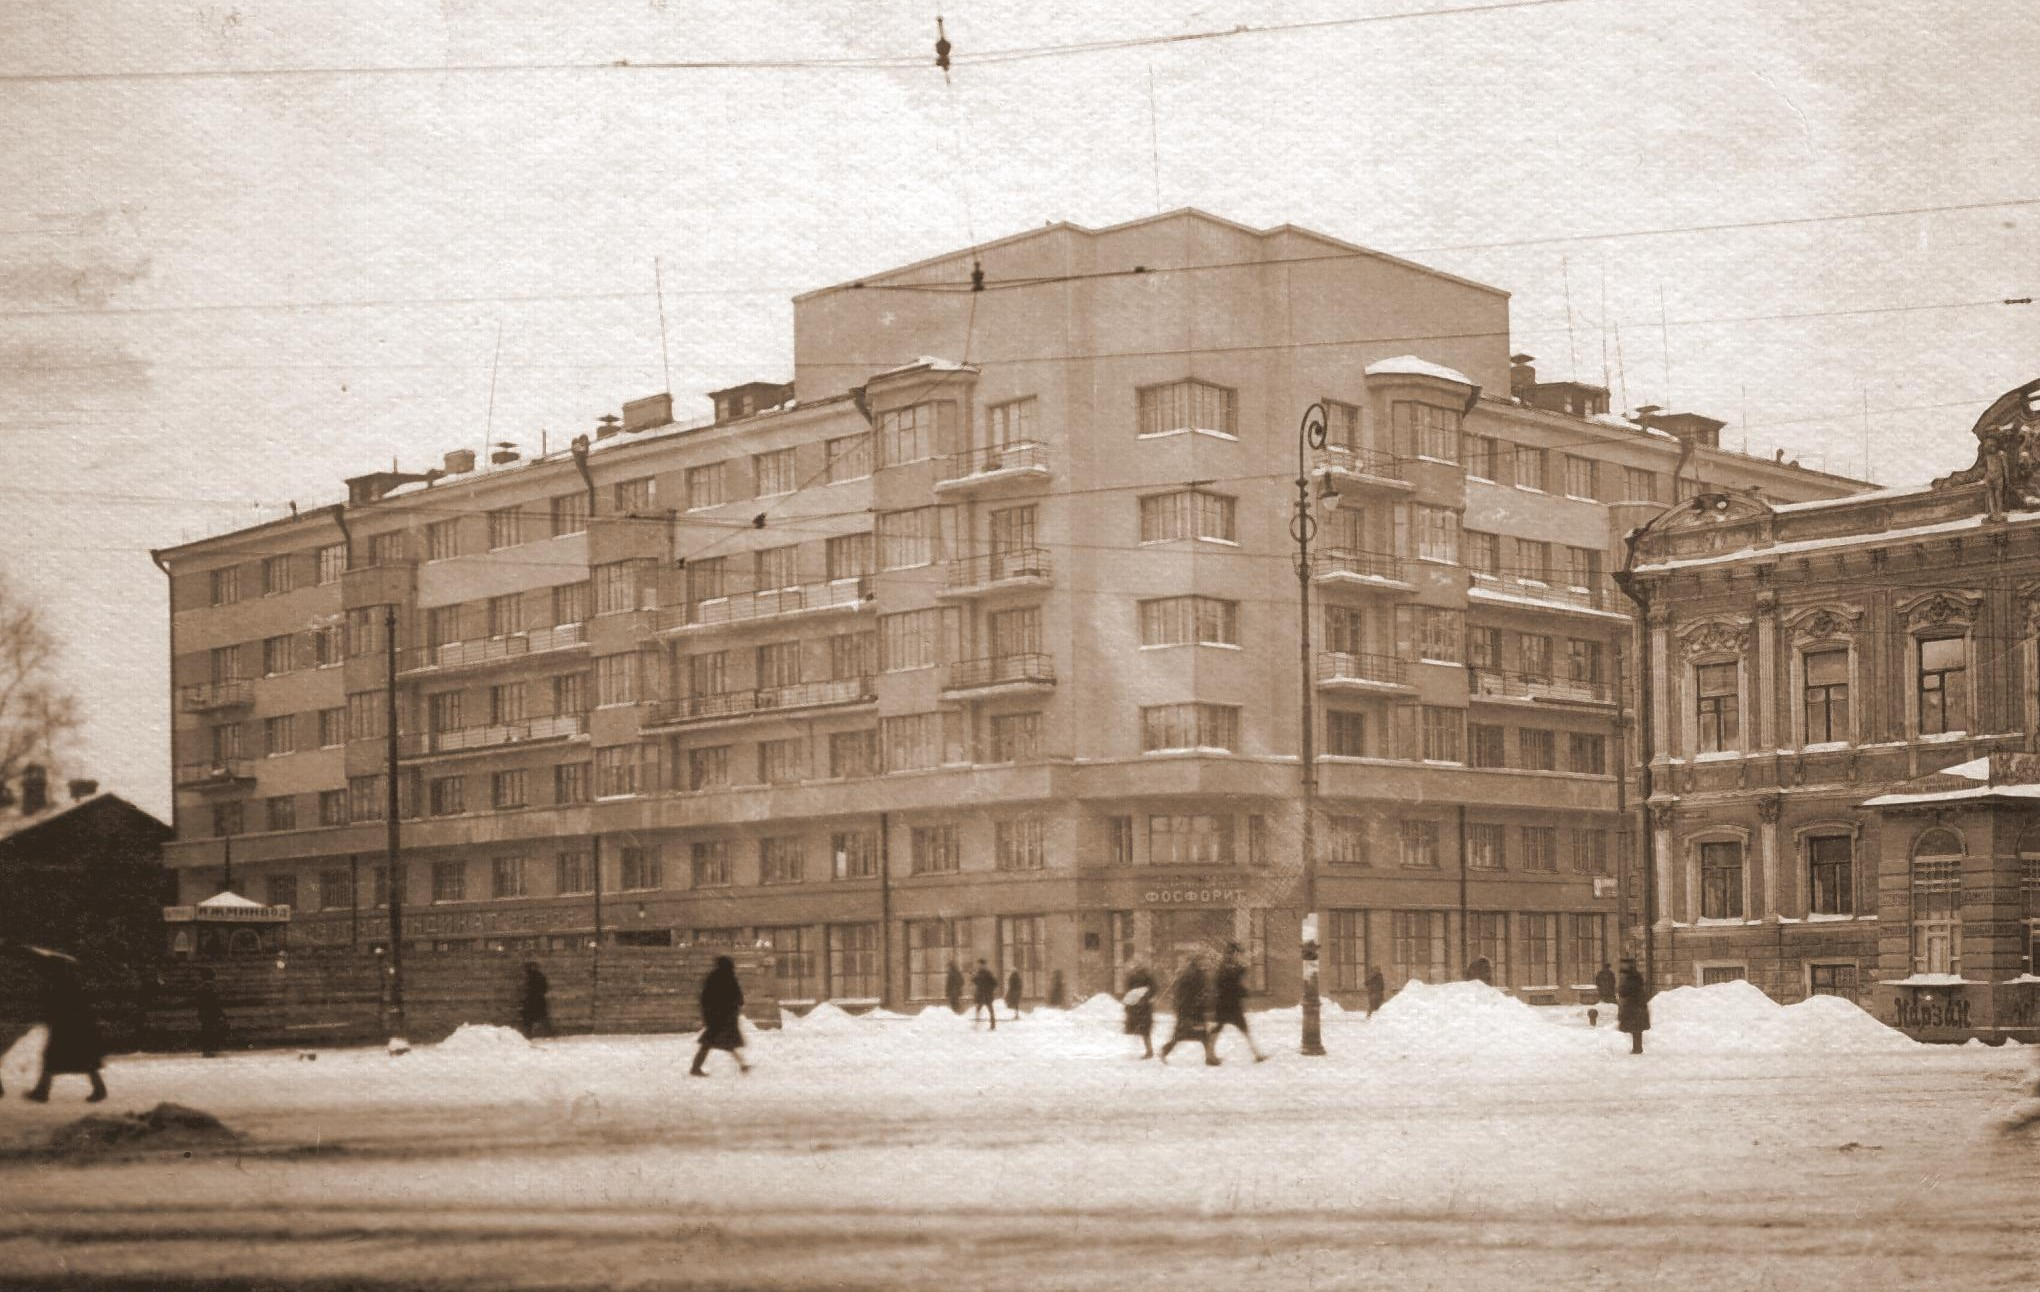
\includegraphics[width=80mm]{inc/2/1}
    \caption{Детский сад нашего дома (1936 или 1937 год). Нижний ряд: руководительница и ее дочь, Таня Меньшикова, Таня Сиротина, примкнувшая девочка, Ксения Варзар, Ира Ильинская; верхний ряд: Марик Миникс, Лева Меньшиков, Юра Райский, Олег Гриневский, два примкнувших парня, Ира Каменская, директор детсада.
}
\end{figure}

\begin{figure}
    \begin{minipage}[h!]{49mm}
        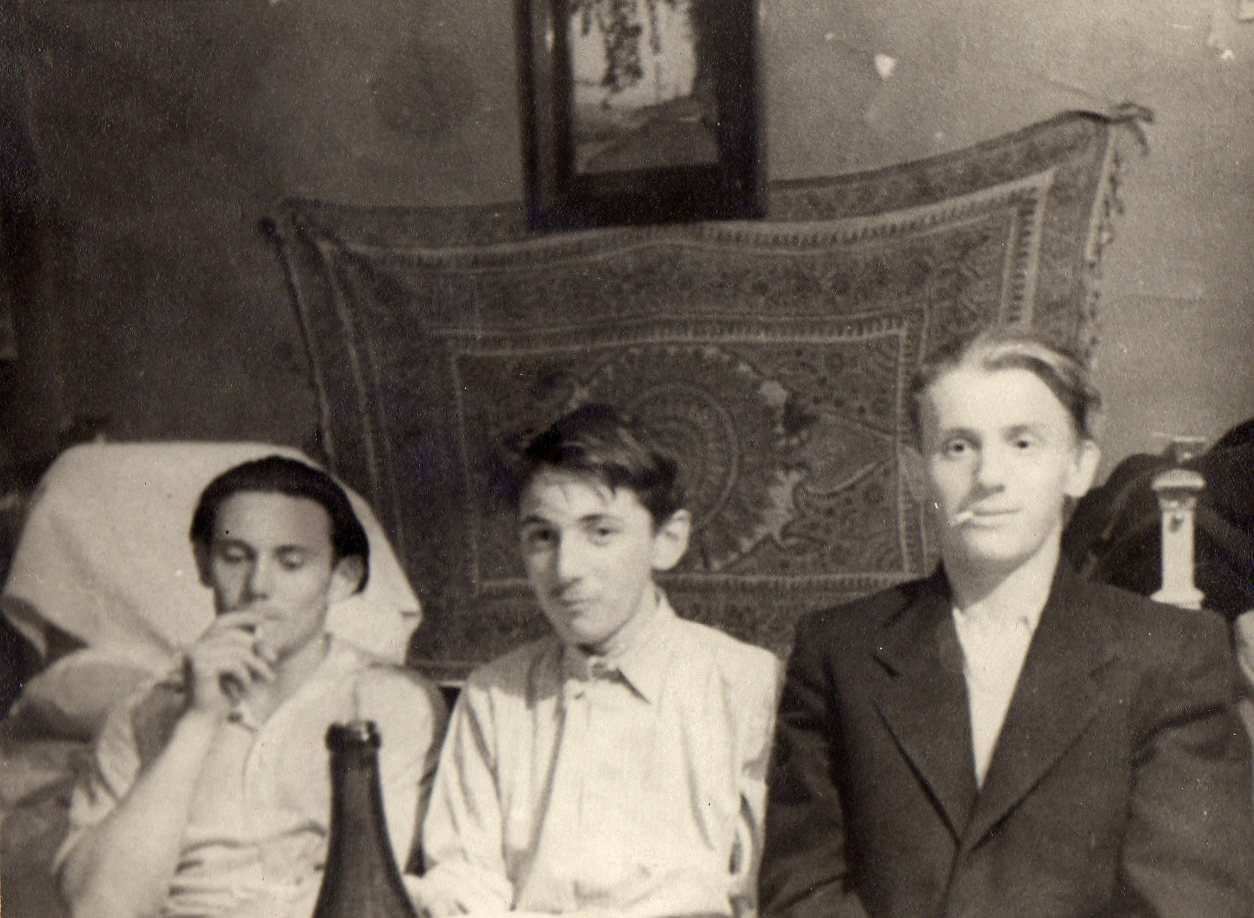
\includegraphics[width=\linewidth]{inc/2/4}
        \begin{footnotesize}\textit{Володя Литвинов, Игорь Петров, Сергей Дивильковский. Около 1950г.}\end{footnotesize}
    \end{minipage}
    \hspace{5pt}
    \begin{minipage}[h!]{25mm}
        \includegraphics[width=\linewidth]{inc/2/2}
        \begin{footnotesize}\textit{Таня Меньшикова и Ира Каменская}\end{footnotesize}
    \end{minipage}
\end{figure}

\begin{figure}[h!]
    \includegraphics[width=80mm]{inc/4/1}
    \caption{«Старшие ребята» (1946 год). Нижний ряд: Зоя Карпухина, Люция Фролова, Ксения Варзар, Галя Давыдова, Неля Тарасова, Алла Пивень; средний ряд: Светлана Факторович, Игорь Петров, Коля Фролов, Шурик Штернберг, Леон Кузнецов, Ира Каменская; верхний ряд: Миша Медников, Боря Коваль, Лиля Бирюкова, Олег Гриневский, Сергей Дивильковский. }
\end{figure}

\begin{figure}[ht]
    \includegraphics[width=100mm]{inc/6/2}
    \caption{На 50-летии Т. В. Меньшиковой. Сидят: Лев Меньшиков, Ксения Варзар, Зоя Карпухина (Литвинова), Игорь Петров, Татьяна Мньшикова, Лиля Буженова, Алла Пивень. Стоят: N.., Борис Шипилов (муж Аллы), Борис Коваль, Люся Осипова, Галя Прейс, Витя Прейс, Володя Литвинов, Шурик Шитернберг.}
\end{figure}

\begin{figure}[h!]
    \noindent
    \begin{minipage}{65mm}
        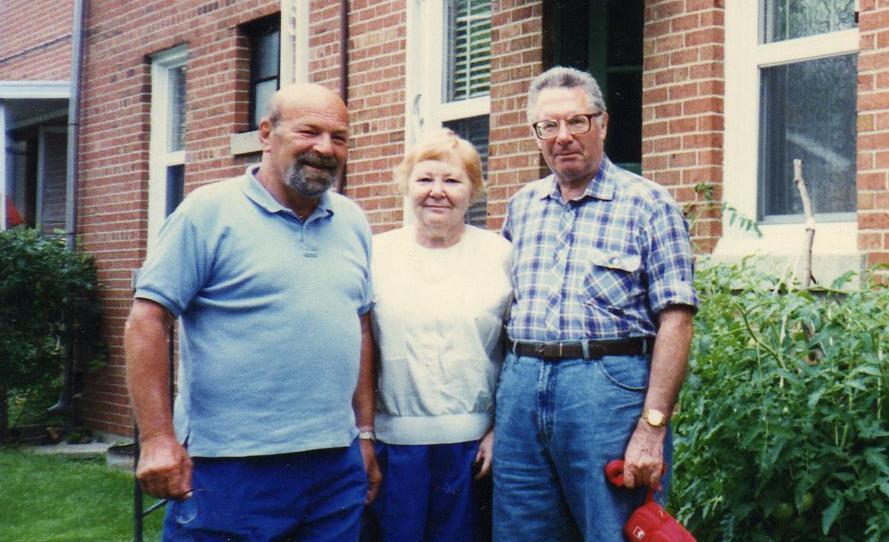
\includegraphics[width=\linewidth]{inc/6/4b} \begin{footnotesize}\textit{Шурик Штернберг, Лиля Бирюкова и Витя Прейс в 1966 г. }\end{footnotesize}
    \end{minipage}
    \hfill
    \begin{minipage}{55mm}
        \includegraphics[width=\linewidth]{inc/6/3} \begin{footnotesize}\textit{Зоя Карпухина (Литвинова) и Витя Прейс.}\end{footnotesize}
    \end{minipage}
\end{figure}

\onehalfspacing

{\raggedleft В связи с отъездом Шурика и Лили.

}

\begin{multicols}{2}

\itshape
    
    \noindent
    Сиреневый туман \\
    Опять благоухает \\
    И годы-облака \\
    Плывут за горизонт \\
    \vfill
    \columnbreak
    \noindent
    А жизнь летит вперед,\\
    Она не понимает,\\
    Что ты уже не та,\\
    И я уже не тот. \\
    \vfill
    \columnbreak
    \noindent
    Как много лет назад\\
    Мы были молодыми\\
    И создавали свой\\
    Счастливый детский мир\\
    \vfill
    \noindent
    Писали <<Вундеркинд>>,\\
    немного воровали,\\
    Неслись за табаком\\
    В общественный сортир\\
    \vfill
    \noindent
    Курили мы во ВШАх,\\
    На крышах загорали,\\
    К Татьяне на балкон\\
    Валились как десант.\\
    \vfill   
    \noindent 
    По штанге на руках\\
    Взбирались к Бирюковой\\
    И Люции втроем\\
    Развязывали бант.\\
    \vfill
    \noindent
    И дружно всей семьей\\
    Потискивали нежно\\
    Но чьи? Когда? И как?\\
    -- Общественный секрет.\\
    \vfill
    \noindent
    На все, что сверх того,--\\
    Почти что добровольно\\
    Мы наложили свой \\
    Монашеский запрет.\\
    \vfill
    \noindent
    Как было хорошо!\\
    Как искренне дружили!\\
    Как пели во дворе,\\
    Пугая старый дом!\\
    \vfill
    \noindent
    Всё было впереди:\\
    Семья, работа, годы...\\
    Но всё это уже\\
    Случилося потом.\\
    \vfill
    \noindent
    Конечно, не вернешь~--\\
    Что было, то уплыло,\\
    Но молодость свою\\
    Нам не забыть вовек.\\
    \vfill
    \noindent
    Ведь именно тогда\\
    Мы родились вторично,\\
    Как братский и родной\\
    Единый Человек!\\
    \vfill
    \noindent
    Уже кого-то нет,\\
    И кто-то уезжает,\\
    И в XXI-ый век\\
    Придут не все из нас.\\
    \vfill
    \noindent
    Но молодость была,\\
    Она не умирает,\\
    До гробовой доски\\
    Сопровождая нас!\\
\end{multicols}
%\end{scriptsize}
\vspace*{-5mm}

{\raggedleft Борис Коваль 20.05.1994 

}

\newpage

\begin{figure}[h!]
    \begin{minipage}{80mm}
    \includegraphics[width=80mm]{inc/6/1}
    \textit{\footnotesize{2004 г. Борис Коваль, Игорь Петров, Люция Фролова, Тамара Зайцева, Леон Кузнецов.}}
    \end{minipage}
\end{figure}

\begin{figure}[h!]
    \begin{minipage}{80mm}
    \includegraphics[width=80mm]{inc/5/1}
    \textit{\footnotesize{Олег Гриневский, Борис Коваль, Леон Кузнецов, Тамара Зайцева, Люция Фролова, Татьяна Меньшикова, Игорь Петров, Ксения Варзар}}
    \end{minipage}
\end{figure}

\begin{figure}[h!]
    %\begin{minipage}{80mm}
    \includegraphics[width=80mm]{inc/4/2}
    \caption{Борис Коваль, Олег Гриневский, Тамара Зайцева, Наталия N, Леон Кузнецов, Зоя Литвинова (Карпухина), Татьяна Меньшикова накануне всеобщего 80-летия.}
    %\end{minipage}
\end{figure}

\newpage

\begin{center}
{\largeВсеобщее восьмидесятилетие}
\end{center}
\vspace{-10pt}
\begin{figure}[h!]
    \begin{minipage}{80mm}
    \includegraphics[width=80mm]{inc/7/3}
    \textit{\footnotesize{Ксения Варзар, Олег Гриневский, Татьяна Меньшикова.}}
    \end{minipage}
\end{figure}
\vfill
\begin{figure}[h!]
    \begin{minipage}{80mm}
    \includegraphics[width=80mm]{inc/7/1}
    \textit{\footnotesize{Олег Гриневский, Игорь Петров, Татьяна Меньшикова, Ксения Варзар.}}
    \end{minipage}
\end{figure}
\vfill
\begin{figure}[h!]
    \begin{minipage}{80mm}
    \includegraphics[width=80mm]{inc/7/2}
    \textit{\footnotesize{Юбилей Ксении.}}
    \end{minipage}
\end{figure}

\restoregeometry

\newpage

В возрастной категории ребят нашего двора 1933-1938 годов рождения у Алекксандровской О., Бездетского (Шейнина) О., Досика В., Меньшикова Л., Месежникова Л., Миникса М., Моргунова Б., Пастухова В., Певзнер Э., Плоткина М., Райского Ю. также было много <<приходящих>> друзей: Дмитренко Е., Епишин Ю., Зайчик Ю., Куняева О., Мюллер Г., Панова О., Цимберов Ю., Штарх А. и другие.

Эти компании имели и общих участников (как <<Мир искусств>> и <<Бубновый валет>>), например Алла пивень и Ира Ильинская. То же бывало и у <<младших>>, так: Элла Пивзнер входила и в СД и в компанию представленную на фото четырех.


\indent

\textbf{Из моей книжки <<О людях дома у Красных ворот>> 2010 года.} О своих сверстниках я старался писать в свободном стиле, о себе~-- с подобающей случаю иронией.

Из «Старших ребят» (около 1930 года рождения) нашего двора, вернее, «Союза соединенных дворов» (ССД), постоянные отношения поддерживаю только с Л. Д. Кузнецовым. Встречаемся и созваниваемся мы, правда, редко, но всегда с удовольствием. Он относится к блистательному созвездию личностей, которые «вышли из шинели» ССД. Но о каждом из них напишет, видимо, кто-то из сверстников. Помню, правда, многих и многое, в частности,  что они издавали журнал  «Вундеркинд» (см. Приложение I), были у них и свои денежные знаки (Лондры, Пижмы). В общем – развлекались.

Нам – нашему поколению (около 1933 года рождения) тоже хотелось развлекаться\footnote{Из этого плоколения вышло немало замечательных людей. Да и в то время среди Психов были 3 секретаря комомола и председатель совета дружины разных школ, толковые, многим интересующиеся и многое умеющие ребята.}, и мы организовали «Сумасшедший дом» (СД). Возглавляли его умнейшая и достойнейшая Лёлька Александровская и ее супруг по СД, достойнейший и умнейший Юрка Райский. Каждый из них имел у нас высочайший титул «Почетный псих»; а еще были «Психи первой гильдии», «Члены-корреспонденты СД», просто «Психи» и «Примкнувшие». В одном экземпляре даже был выполнен «Орден почетного члена СД». Это безобразие началось в сорок восьмом, а в пятьдесят     третьем,    когда     Психи     разбежались      по институтам, практически все собрались, чтобы отметить юбилей СД.

У меня как раз оказалось полно свободного времени, поскольку месяца три «провалялся» с сердцем. Поэтому в честь юбилея я сотворил нечто грандиозное: «Гротескную фурнитурию в двадцати четырех Бредах с Прологом и Апофеозом», в которой упоминался почти каждый Псих из СД. Эпиграф был взят из Ю.Д. Райского –   «Лучше переспать, чем недоесть». Пролог начинался достаточно скромно, но с чувством собственного достоинства: 

\newpage
\newgeometry{left=0mm, right=0mm, top=0mm, bottom=0mm}
%\thispagestyle{empty}

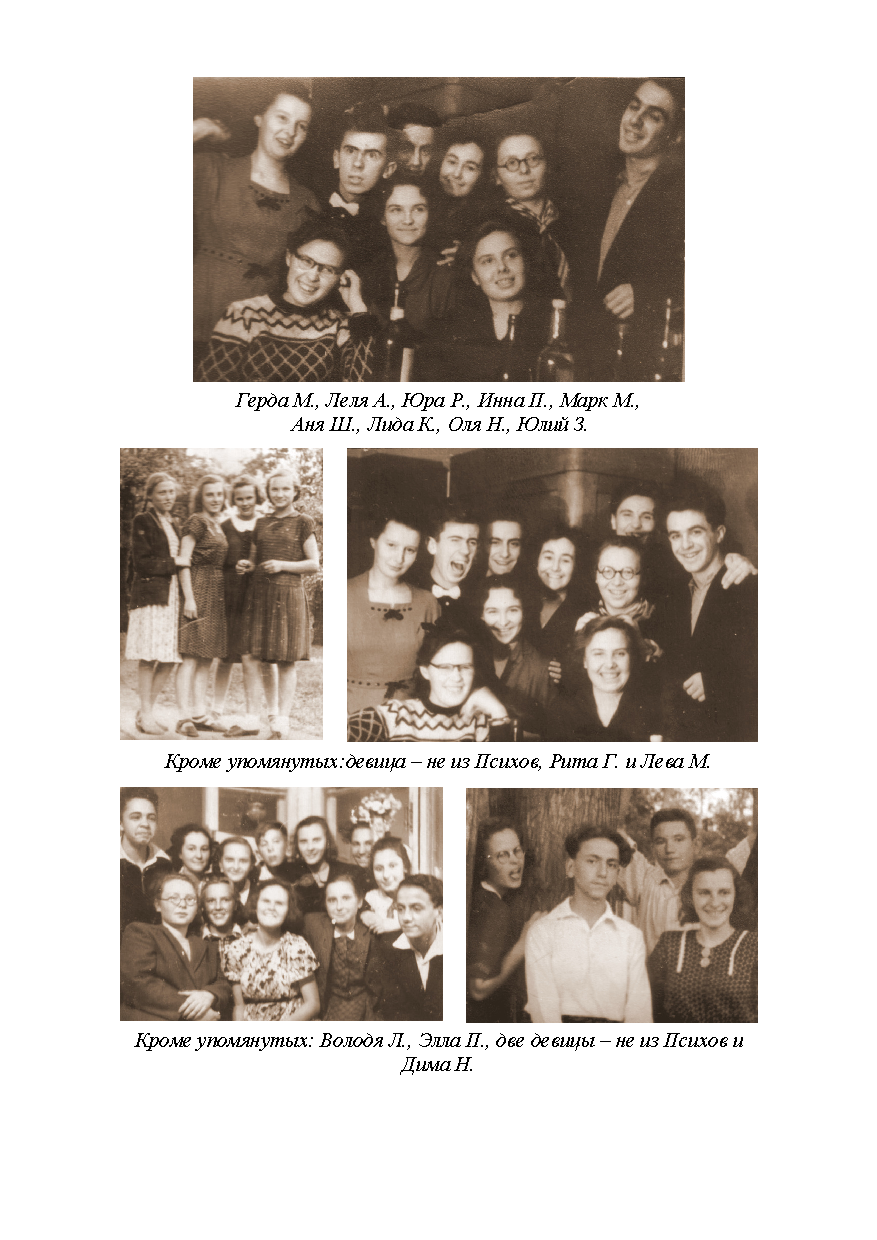
\includepdf[pages=-]{inc/sd1.pdf}


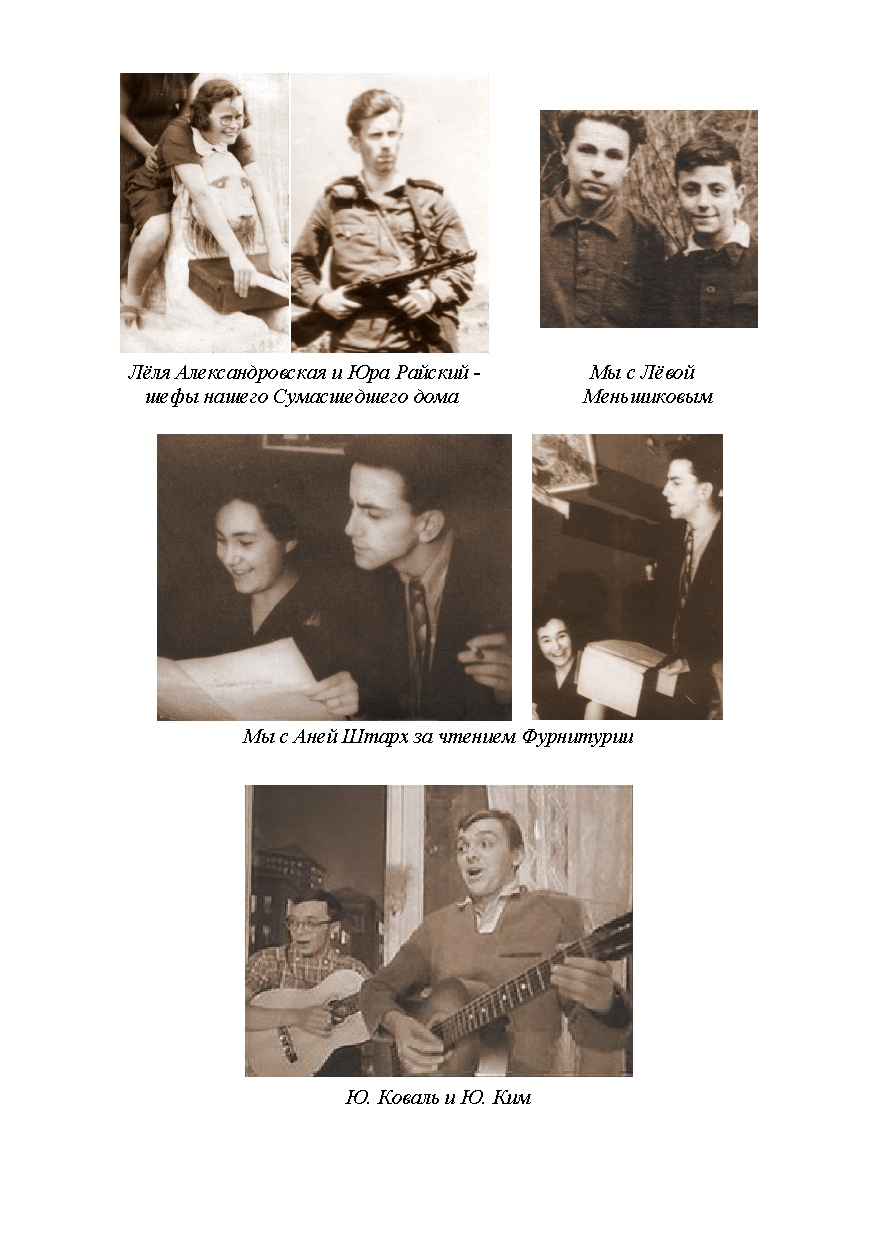
\includepdf[pages=-]{inc/sd2.pdf}

\restoregeometry

{\itshape
    Ничто ни в чем полней не может отразиться,
    
	Чем что-нибудь в стихах моих.
	
	И вот пишу о славном Юбилее,
	
	Чтоб свой навек прославить стих,
	
	И чтоб оставить у потомков
	
	Священной память о Союзе нашем,
	
	Которого и не было, и нет,
	
	И быть не может
	
	В мире краше!
}

\indent

\noindent
Кончалось же совсем пафосно:



{\itshape

    \indent
    
	Наш славный Сумасшедший дом
	
	И чувств и чаяний священная обитель!
}


\indent

Один из Бредов озаглавлен так: «Взгляд на доморощенного идиота с точки зрения высокого полета». Бред, посвященный внутридомному бракосочетанию Психов, включал лозунги-речевки:


\indent

{\itshape
    Псих, не будь трусом,
    
	Не пяться, как рак,
	
	Знай, основы вселенной – 
	
	Семья и брак.
}

\indent 

\noindent
и «Увековечим юбилей повальной женатостью».


В Фурнитурии указано, что единственный лирико-сентиментальный Бред «написан по просьбе\footnote{Просьбы не было, ее поэтически придумал я; фактически же события изложены вполне правдоподобно.}  одного, весьма достойного психа». Имелся в виду Лёвка Меньшиков (Лёвка – уже в школьные годы одаренный радиофизик, вдохновитель, организатор и исполнитель чуть ли не первого школьного радиоузла; Лёлька – см. выше; Женя – ее сокурсница по Университету, жила в общежитии МГУ на Ленинских горах):

\indent

\begin{center}
ЖЕНЕ
\end{center}

{\itshape
Однажды встретившись с тобой у Лёльки,

Я понял сразу – Ты моя судьба…

С тех пор преследует меня Твой образ,

В душе моей смятенье и борьба…

\indent

Я вспоминаю ночь, когда с Тобою

Впервые вышли Мы на улицы Москвы.

Была Ты рядом (!), и с восторженной душою

Я шел, пытаясь замедлять шаги…

\indent

Пусть на метро потом я не попал

И через город весь прошел пешком,

Пусть я чертовски в эту ночь устал,

Но эта ночь осталась лучшим днем!

\indent

}

Кончался этот Бред весьма оптимистично и бравурно:

{\itshape

\indent

	Психоз – явление для нас нормальное,
	
	А психом стал я от любви!
	
	Друзья мои, проблема сексуальная
	
	Рождает страсть, порыв, кипение крови!!

}

\indent

	Еще были краткие анонимные посвящения, например, Лёльке: «Безумие с умом нелегкая задача в общении с друзьями сочетать» и себе: «Желая первым быть, он вечно отстает».


Юрочка Коваль  не был Психом, не входил в СД по молодости лет, но любили его все, как и в зрелые годы, когда он стал большим Литератором. Замечательная «Ковалиная книга» тому подтверждение. А в те времена он всерьез занимался многими важными делами: игрой на гитаре, походами и охотой, живописно-скульптурным творчеством, но только не литературой, правда, в теплой записке в больницу он обещал посвятить мне свой первый опубликованный рассказ. 

В ней, в частности, говорилось: <<... не нужно нам громких слов и слав...>> Так он и прожил всю жизнь: без пустопафосных громогласных изречений и заявлений, без официальной трескучей славы. Но зато в ответ на свое уникальное человеческое обаяние и профессионализм он был со всех сторон окружен глубоким уважением, признательностью, любовью близких людей, друзей, сотоварищей по литературномму и художественному творчеству, учеников, просто знакомых (и интеллигентов-интеллектуалов, и простых селян; и пожилых людей и детей), поклонников и поклонниц его разносторонних талантов.

А в то время он писал талантливые Пародии~-- сами по себе (а-ля Козьма Прутков). Примеры пишу по памяти, так что точность не гарантирована:

\indent

{\itshape
	Один Барклай де Толли гулял по Петрограду.
	
    О Бородинском поле он сочинял балладу.
    
    Э-ге-ге, тра-ля-ля Бородинское поле
    
    Тут рука и нога погуляли на воле.

}

\indent

\noindent
А кончалось так:

\indent

{\itshape
	Э-ге-ге, тра-ля-ля победили французов:
	
	Я, де Толли Барклай и Михайло Кутузов.
}

\indent

\noindent
Еще покрепче:

\indent

{\itshape
	Раз я по полю катался
	
	На власепеде небольшом.
	
	Но власепед под мной сломался,
	
	И я упал о чисто поле лбом.
}

\vfill

\noindent
Кончалась эта история примерно так:

\vfill

{\itshape
	И соловей над мною распинался,
	
	И вынул из ноги валасипедный ключ.	
}	

\indent

\noindent
По-моему, в эпической драме «Канделябры мои канделябры» есть такие незабываемые строки:

\indent

{\itshape
Казалась лилией твоя рябая морда.

Звучал в душе моей рояль-металлолом.
}

\indent

\noindent
Но вершиной этого этапа его творчества стала строфа из какого-то очень значительного произведения:

\indent

{\itshape
	Вышел на поляну Дядиванин гусь…
	
	Я сижу на крыше – хороша ты, Русь!
}

\indent

Сегодня эти милые «суразности» вспоминать и приятно, и грустно, поскольку Юрия Иосифовича Коваля уже нет с нами.

\indent

\textbf{Из моей книжки <<Мои люди>>.} О Б. И. Моргунове, Е. М. Дмитренко, Ю. А. Цимберове

В первой книжке был дан парадный портрет Б. И. Моргунова. Здесь речь пойдет о домашнем Борисе Ивановиче – Боре Моргунове. Я и не пытался дотянуться до него по интеллекту, эрудиции, потенциалу, но мы всегда были, до смешного, принципиальными, непримиримыми соперниками в любых игрищах: в шахматы, в бильярд, в домино, в карты, в мячик (цель – попасть мячиком последовательно во все промежутки между ступеньками лестницы, приставленной к дачному дому). На старости лет мы старались «играть вничью», чтобы не огорчать друг друга. С другой стороны, мы очень часто по самым разнообразным вопросам, по оценкам событий, явлений, произведений искусства, даже людей, были настроены на общую волну, или находили интересные компромиссы. Были, конечно, и исключения. 
	
	Как всякий блестящий ум, он порой был неудовлетворен собой. К окружающему миру, видя его несовершенство, он относился снисходительно. Всегда весьма активный в делах (написание книг, статей, подготовка к лекциям, работа с аспирантами), он был весьма инерционен в быту. Зная очень многое о театре, музыке, живописи, он долгие годы ограничивался прослушиванием и просмотром записей. 
	
	Продолжительные прогулки по лесу, пока позволяли ноги, он очень любил. Видимо, такие прогулки снимали стрессы, накопившуюся усталость, моральное напряжение. В лес, вообще на даче, он надевал самые простые, привычные, часто совсем не новые, но очень удобные ему вещи. Поэтому утром, когда он собирался на лекции и брился, надевал костюм и рубашку с галстуком, контраст выглядел разительно, поскольку из дома выходил не расслабленный отдыхающий «Боренька, серенький», а собранный, даже сконцентрированный, уже озабоченный делами предстоящего дня профессор Б. И. Моргунов.
	
	Был он по натуре человеком сосредоточенным, при всей своей общительности – порой даже замкнутым и грустным, но через минуту, обладая молниеносной реакцией, мог быть блестяще остроумен. Только один пример из множества.
	
	Мы остались ночевать на даче. Под утро, часа в четыре, у меня случилась судорога, и я, видимо, достаточно громко закряхтел. Б. И. открыл глаза, изрек

\indent

{\itshape
		И только солнце рассвело,
		
		Как ногу Миниксу свело
}

\indent

и заснул. Вообще чувство ритма: поэтического, музыкального, было характерно для него и часто проявлялось самым неожиданным образом.

	Еще несколько примеров его стихоизвержений. «Мама Светочка» опрометчиво положила коробку с десятком яиц на кресло, кто-то на них сел, по-моему, сам Б. И., который тут же запел на знакомый всем мотив: 

\indent

{\itshape
		Я раздавил коробку с яйцами,
		
		Яйцами, яйцами…
}

\indent

Кто-то из нас поймал от знакомой кошки лишай… и заразил Бориса, который тут же сочинил:

\indent

{\itshape	
		Лишаями покрыто все тело,
		
		Больно голову, ноги и грудь.
		
		Это Миниксов подлое дело,
		
		В морду дать ты им, друг, не забудь.
}

\indent		

	Лежит на диване, пишет статью (нормальное дело, в порядке вещей). Видимо, что-то не ладится. Вдруг раздается душераздирающий вопль (на «позывной» мотив из пятой Бетховена):

\indent

{\itshape
		Ходит муха по стене,
		
		Хлопнем муху по спине…
}		

\indent

Теперь примеры более капитальных творений. Первую свою вышедшую статью он подписал мне так:

\indent

{\itshape
		Тот первый блин,
		
        Который комом,
        
        Дарю друзьям я
        
        И знакомым.
}

\indent

\noindent
А первую монографию так:

\indent

{\itshape	

	Рад доложить я Марюленьке\footnote{Так меня звала с детства мама. Ирушка Моргунова, узнав об этом, стала называть меня <<Малюленькой>>.} - Марку:

	Труд капитальный
	
	Пошел не насмарку.
	
	В общем, я выдержал нужную марку,
	
	Жаль, что найдешь ты, однако, помарку.
}	

\indent

О Борисе Ивановиче можно говорить бесконечно.

Женя Дмитренко и Юра Цимберов были первыми – с младших классов, самыми верными друзьями Бори Моргунова. Юра обладал огромным обаянием. Трудно себе представить человека более искрометного и добросердечного. К сожалению, он рано ушел из жизни.

С Женей и его женой Ларой мы сблизились еще при Боре. А его уход особенно сплотил нас. Евгений Михайлович Дмитренко – талантливый математик, выпускник механико-математического факультета МГУ, уже с юношеских лет был вполне сформировавшимся человеком, самостоятельно мыслящим, трезво оценивающим жизненные обстоятельства, твердо стоящим на ногах, придерживающимся вполне определенных взглядов. Борис Иванович очень высоко оценивал его творческий потенциал.

Он рано полюбил музыку и, особенно, живопись. Был знаком со многими молодыми талантливыми художниками. Со временем начал приобретать их картины, которые теперь стали классикой. Больших денег у него не было, но интересную коллекцию он собрал.

Сейчас у него огромное собрание записей музыкальной классики всех времен, направлений, стилей и форм. Свободных стен нет: масса книг, самых различных, в основном – классика.

У него очень хорошие, совершенно самостоятельные, отношения с моим сыном; эта эстафета перешла от Бориса Ивановича.

Мы сравнительно часто встречаемся, всегда – с удовольствием. Я часто бываю тронут его вниманием и теплотой. Недавно мы с женой и сыном были на его семидесятипятилетии. Были и Моргуновы – Светлана Сергеевна и Ира.


\indent

Ниже представлены компании ребят нашего двора середины тридцатых и середины сороковых годов рождения.

\begin{figure}[h!]
    \noindent
    \begin{minipage}[t][65mm]{45mm}
        \includegraphics[width=30mm]{inc/9/1}
        
        \begin{footnotesize}\textit{NN, Таня Пантина, \\ Катя Каплун, Элла \\ Певзнер. 1948 г.}\end{footnotesize}
    \end{minipage}
    \hfill
%    \vspace{-20pt}
    \begin{minipage}[t][65mm]{61mm}
        \includegraphics[width=61mm]{inc/fontan} \begin{footnotesize}\textit{Так наш фонтан выглядит сегодня}\end{footnotesize}
    \end{minipage}
\end{figure}

\vspace{-20pt}

\begin{figure}[h!]
    \thisfloatsetup{capbesideposition=right}
    \fcapside[\FBwidth]{\includegraphics[width=54mm]{inc/9/2}}{    \caption{Стоят: Галя Пантина, Галя Давыдова, Галя Столяревская; сидят: NN, Владик Каплун, NN, Боря Пенько, Володя Пастухов. Начало 50-х.}}
    

\end{figure}

\newpage

Сегодняшние ветераны ($80\pm5$лет) хорошо помнят, что никакого <<духа Рублевки>> в нашем дворе никогда не было. важны были не должность и достаток родителей, а твоя собственная сила, ловкость, голова, увлечения, умения.

Потом пришла пора зрелости, профессионализма, мудрости; постепенно мы стали <<хозяевами жизни>>. А вокруг бушевал XX век, появлялись и требовали своего все новые и новые поколения, и, наконец, грянул XXI век. В результате <<все изменилось до полной неузнаваемости>> (Рей Бредбери).

А молодежь? Она не хуже и не лучше, чем в наши времена. Она другая.

\newpage


Ниже в алфавитном порядке приведены примеры выдающихся людей, выросших в наше дворе. Подчеркиваем ~-- это только примеры. Замечательных людей среди жильцов нашего дома, разумеется, гораздо больше\footnote{Например, семья первопоселенцев Займовских: дед, профессор-лингвист, работал на семи языках, сын~-- физик, действительный член АН СССР, внук~-- талантливый инженер.} (у всех, кроме Дивильковского, указаны должности, которые они занимали в различные годы).

\textit{В. А. АНДРЕЕВ.} Народный артист СССР, Художественный руководитель Театра им. Ермоловой, ранее~-- Малого театра, профессор.

\textit{О. А. ГРИНЕВСКИЙ.} Член коллегии МИД, Чрезвычайны и полномочный посол СССР и России, руководитель и участник ряда делегаций страны на международных переговорах, профессор. Автор восьми книг, изданных в России, Швеции, Германии, соавтор двух книг, выпущенных в США. Книга <<Перелом. От Брежнева к Горбачеву>> вышла в 2004 г. (ОЛМА-ПРЕСС).

\textit{С. И. ДИВИЛЬКОВСКИЙ.} Окончил МГИМО и Дипломатическую академию. Советник МИД РФ 1-го класса. Орденоносец.

1967--1970~гг. Советник Посольства СССР в Демократьической республике Вьетнам (связь с Южным Вьетнамом);

1970--1980~гг. Референт международного отдела ЦК КПСС (сектор Вьетнама);

1980--1982~гг. Советник  Представительства СССР при ООН в Нью-Йорке;

1982--1985~гг. Советник Посольства СССР в Вашингтоне;

1986--1989~гг. консультант международного отдела ЦК КПСС.

\textit{Б. И. КОВАЛЬ.} Главный научный сотрудник Института Латинской Америки РАН, профессор, доктор исторических наук, действительный член РАЕН, академик Международной академии португальской культуры, заслуженный деятель науки РФ. Автор цикла фундаментальных трудов по проблемам Латинской Америки и общей теории социального развития.

\textit{Ю. И. КОВАЛЬ.} Художник, превосходный знаток русского языка и русской природы, талантливый писатель:

<<А у Коваля, как ни у кого, открытость и доброжелательность сразу видны, что в прозе, что в характере. Какой человек!>>, << ...Очень вкусная проза>> (Юлий Ким);

<< ...его юмор~-- это правда, не требующая никаких доказательств>> (Фазиль Искандер);

<<Я думаю, что он один из самых чистых служителей русского слова...>> (Андрей Битов);

<<Он был необычайно талантлив... артистичен и обаятелен>> (Марина Тарковская).

Добрые слова о Ю. Ковале, о героях его книг говорили Р.А.~Быков, П.Н. Фоменко, А.Б. Фрейндлих. Кто-то очень здорово назвал его то ли <<поэтом среди прозаиков>> то ли <<поэтом в прозе>>. В его Мастерской часто встречались Б. Ахмадулина, Ю. Визбор, В. Высоцкий, Ю. Ким  и многие другие замечательные люди.

\textit{Г. Д. КУЗНЕЦОВА.} Главнй научный сотрудник Института высшей нервной деятельности и нейрофилиологии РАН, доктор биологических наук, профессор. автор трех монографий и около 150 статей.

\textit{Л. Д. КУЗНЕЦОВ.} Заведующий лабораторией ГИАП (технология синтеза аммиака и катализаторов этого процесса). Кандидат технических наук. Лауреат премии Правительства РФ в области науки и техники. Лауреат Госпремии Украины. Видный изобретатель (более 20 Авт. свид. СССР).

\textit{Б. И. МОРГУНОВ.} Доктор физико-математически наук, профессор, автор пятнадцати книг. Талантливый исследователь и педагог: подготовил двух докторов и около 10 кандидатов физ-мат наук. Человек мощного интеллекта и исключительной эрудиции (деятельной, творческой) в различных областях Знания и Культуры.

\textit{М. М. ПЛОТКИ.} Зам. директора Института социальной педагогики Российской Академии образования, руководитель Центра профессионального образования, доктор педагогических наук, профессор.

\textit{В. Б. ПРЕЙС.} Главнй педиатр Минздрава РСФСР.

\textit{Ю. Я. ЯХНИНА.} Известный переводчик художественной литературы с французского и шведского языков,  Командор Ордена Полярной Звезды - таким орденом от имени короля Швеции награждают иностранцев за  заслуги перед Шведским Королевством.
